\documentclass[a4paper]{article}
\usepackage[utf8]{inputenc}
\usepackage{graphicx} % Required for inserting images
\usepackage[italian]{babel}
\usepackage{gensymb}
\usepackage{array}
\usepackage{amsmath}
\usepackage{hyperref}
\usepackage{siunitx}
\usepackage{caption}
\usepackage{systeme}
\usepackage{wrapfig}
\usepackage{placeins}


\makeindex
\setlength{\parindent}{0pt}

\title{Misura del Modulo di Young di un Cavo di Acciaio}
\author{Francesco Giuliano Rossi}
\date{Maggio 2025}

\begin{document}
\maketitle
\tableofcontents

\begin{abstract}
    In questa esperienza si vuole misurare sia il modulo di Young per un filo di acciaio. 
\end{abstract}

\section{Introduzione Teorica}
\subsection{Introduzione Generale}
Ogni materiale, se sottoposti a sollecitazioni come trazione, compressione, torsione, o scorrimento si deformano. Questa deformazione è detta elastica se il corpo torna allo stato originale quando vengono a meno le forze che causano la deformazione. Tuttavia, ogni oggetto ha un limite che dipende dal materiale, temperatura, dal tipo di deformazione e vari altri fattori, detto limite elastica. Se si supera questo limite, si arriva al cedimento strutturale del materiale. Tutte le deformazioni elastiche seguono la legge di Hooke, ovvero una relazione di proporzionalità tra sollecitazioni e deformazioni. La costante che lega queste due quantità, è chiamata la costante elastica $k$. Come detto prima, dipende dal materiale, temperatura, lunghezza lungo la direzione di trazione e sezione trasversa rispetto a tale direzione, quindi si può scrivere la costante elastica come funzione di vari variabili $k(materiale,T,S,L)$. Si osserva che a parità di lunghezza, la costante elastica cresce in modo proporzionale alla superficie, e quindi si ha $k(S,L)\propto S$ e inoltre decresce in modo inversamente proporzionale alla lunghezza, esprimibile attraverso la relazione $k(S,L)\propto \frac{1}{L}$. 

\subsection{Modulo di Young}
Usando le relazioni ottenute nella sezione precedente, si ha che

\begin{equation}
    F=k(S,L)\Delta L \implies \frac{F}{S} = \frac{kl}{s} \frac{\Delta L}{L}
\end{equation}
e possiamo introdurre due nuove quantità, lo sforzo (stress): 

\begin{equation}
    \delta = \frac{F}{S}
\end{equation}
e il coefficiente di deformazione, anche detto allungamento relativo (strain):

\begin{equation}
    \epsilon = \frac{\Delta L}{L}
\end{equation}
Unendo le due relazioni ottenute, si può scrivere 

\begin{equation}
    \sigma S = k(S,L)L \epsilon \implies \sigma = \frac{k(S,L)L}{S}\epsilon
\end{equation}
Usando questa relazione, si può fare un grafico dello stress in relazione dello strain e definire il gradiente del grafico come $E_m(T) = \frac{k(S,L)L}{S}$ ovvero il modulo di Young. Questa grandezza ha unità $Nm^{-2}$, ovvero Pascal. In questo modo il modulo di Young dipende solo dal materiale usato e la temperatura. \\
Quando un oggetto viene schiacciato o allungato, la sua dimensione trasversale cambia. Questo viene espresso attraverso la legge di Poisson 
\begin{equation}
    \frac{\Delta r}{r} = -v \frac{\Delta L}{L}
\end{equation}
dove v è il coefficiente di Poisson, una quantità adimensionale. 

\begin{wrapfigure}{l}{0.35\textwidth}
    \vspace{-0.50cm}
    \begin{center}
    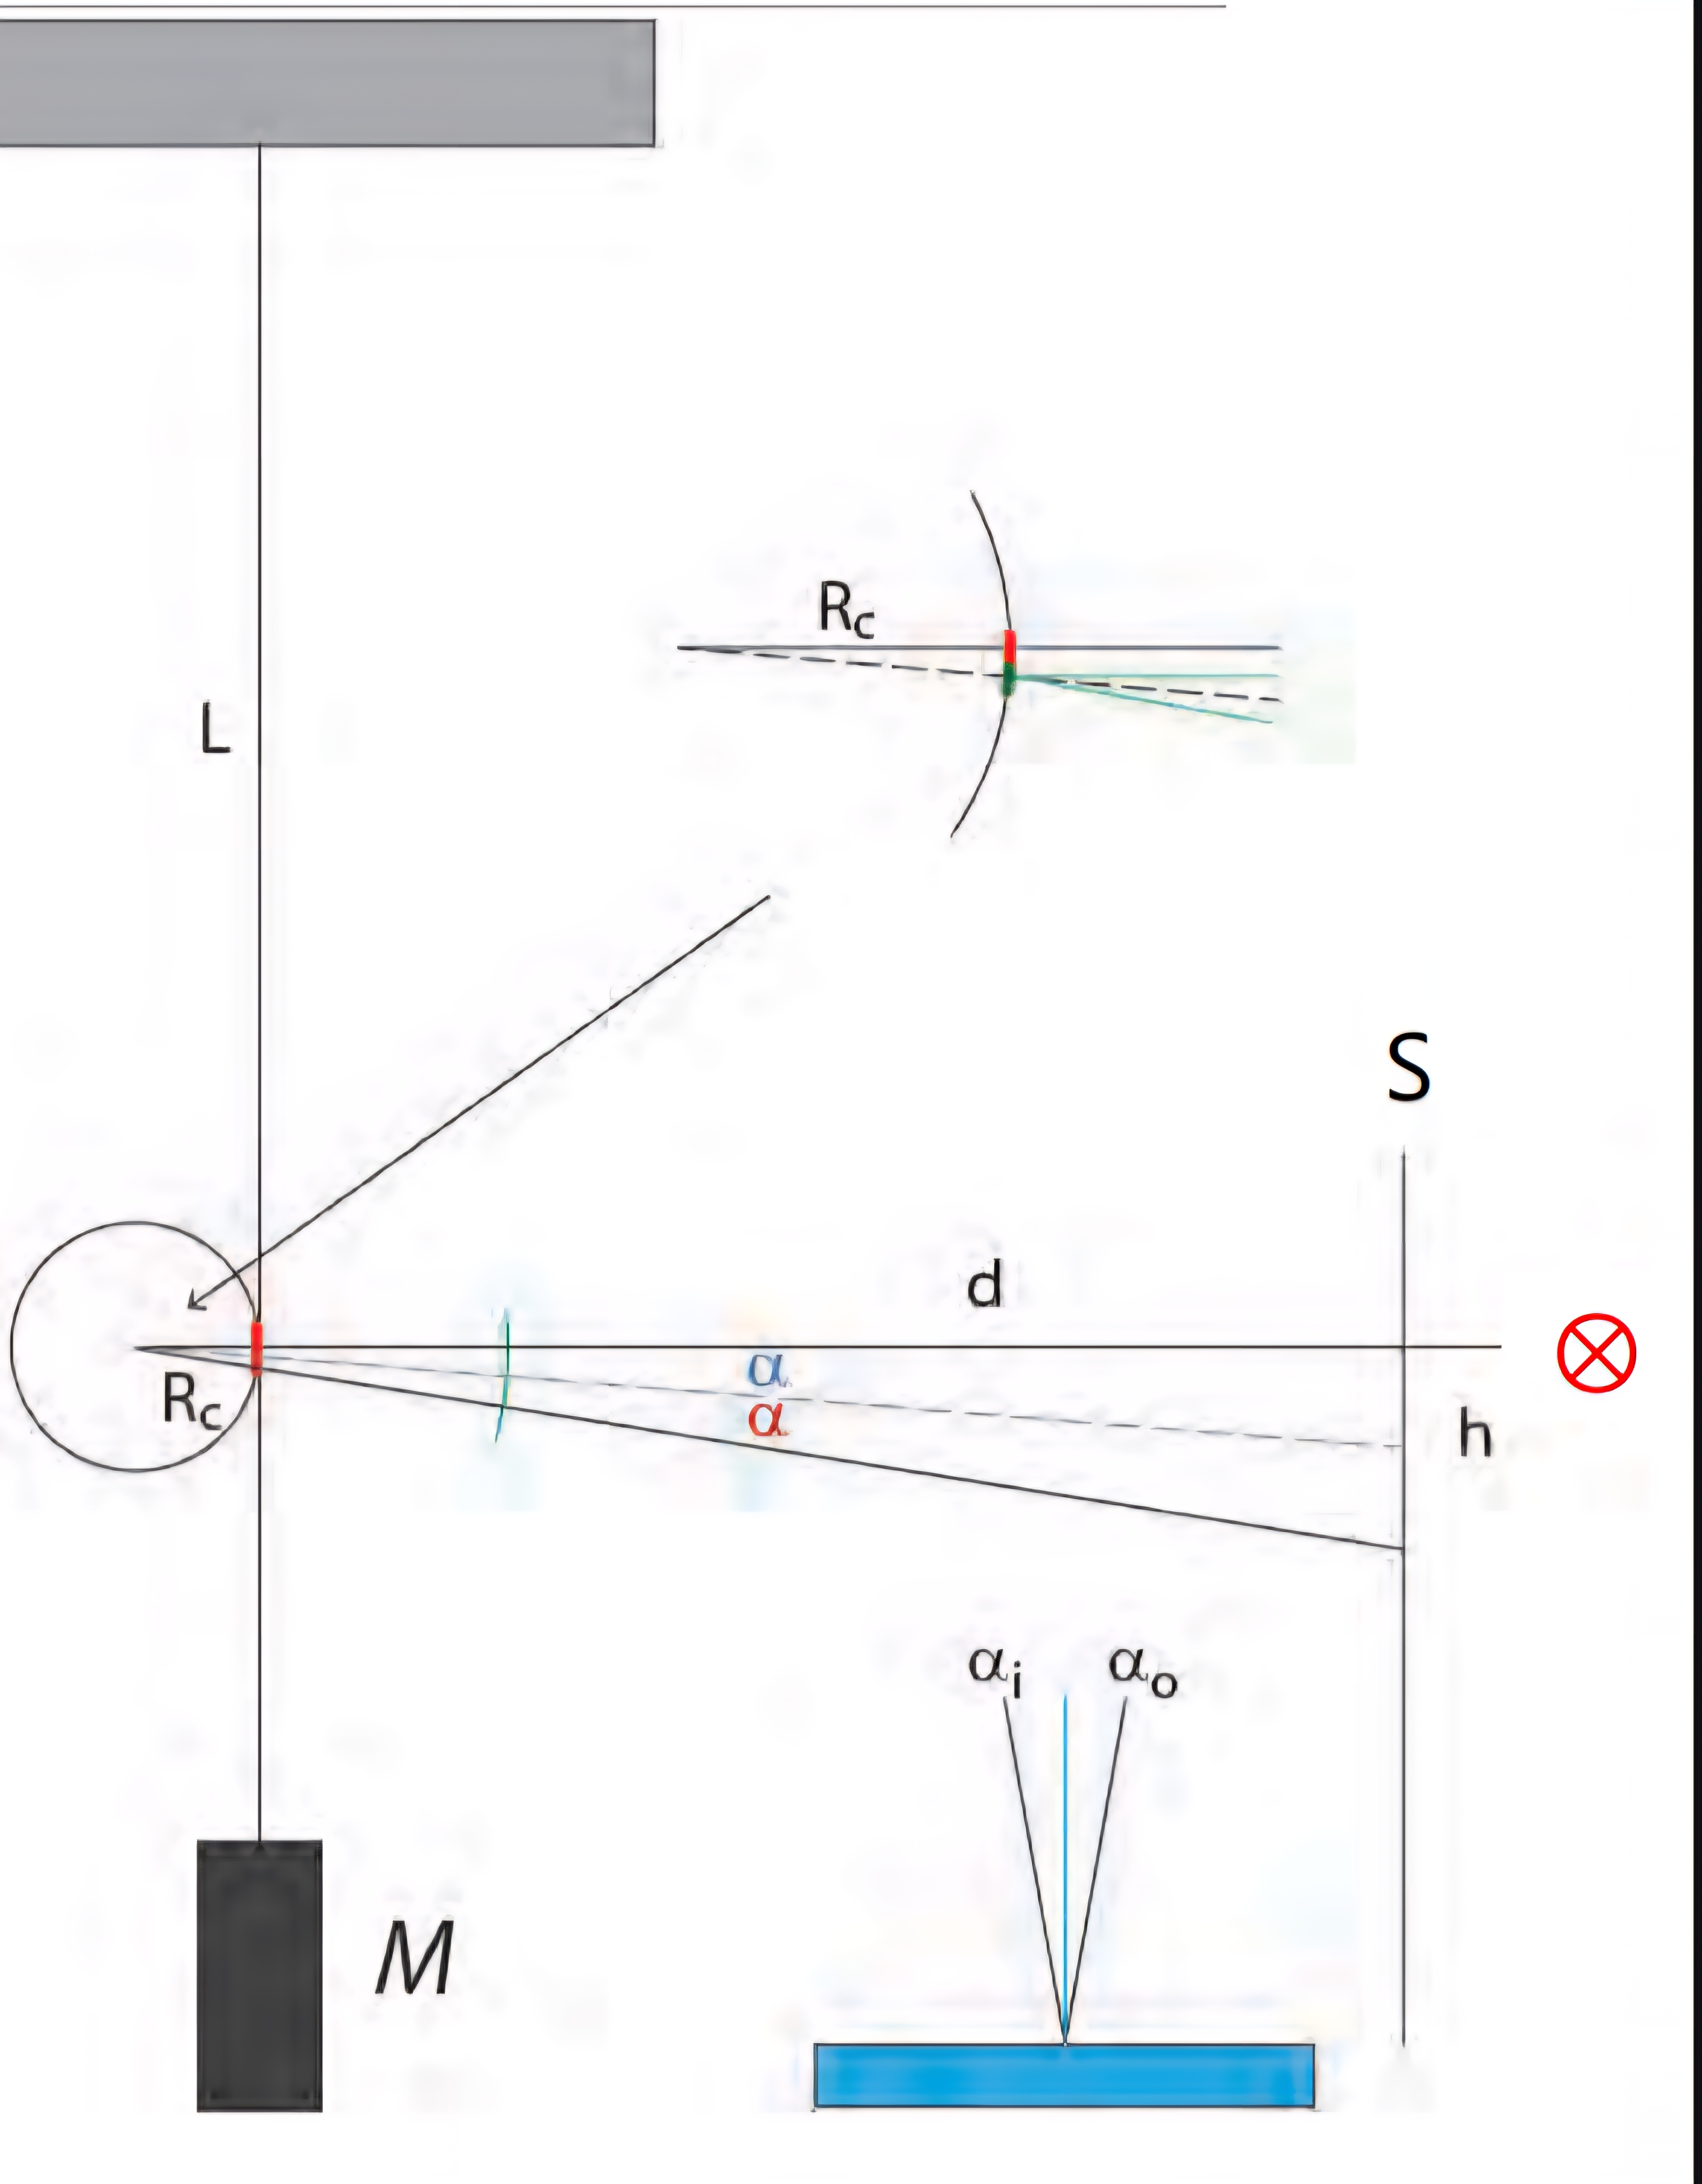
\includegraphics[width=0.35\textwidth, trim={0 0 4cm 0},clip=true]{fotoyoung/levaottica.jpg}
    \end{center}
\end{wrapfigure}


Se si considera un filo di volume costante, la variazione di volume $\Delta[\pi r^2L] = 0$ e il coefficiente di Poisson risulta $v = \frac{1}{2}$. Per un materiale non perfettamente elastico, risulta che $v \leq 0.5$. Questo vuol dire che quando un materiale viene allungato, la sezione trasversale si restringe e il volume totale aumenta. 
Usando questa proprietà, possiamo sfruttare la leva ottica, come mostrato in figura. 


Questo è un apparato costituito da un filo di diametro $D_f$, fissato superiormente a un supporto, che dopo una certa distanza $L$, è rotolato attorno un cilindro di raggio $R_c$. All'estremità inferiore è appeso un piattello su cui si possono mettere delle masse campioni $M_i$. A una distanza $d$ si ha la scala graduata opposto al cilindro e dietro una sorgente di luce che produce un fascio di luce che viene riflesso da uno specchio collocato sul cilindro. Questo fascio di luce si può leggere su una scala graduata per ottenere $h$. 

È molto importante tarare questo strumento nel modo giusto. Questo deve essere fatto con una massa tara per assicurarsi che il filo sia teso. Dopo che più masse sono poste sul piattello, il cilindro ruota, e usando l'altezza $h$ segnato, si può ricavare l'angolo di rotazione $\theta$ attraverso la relazione 
\begin{equation}
    \tan(\theta) = \frac{h}{d}
\end{equation}

e quindi l'angolo risulta, con l'approssimazione per angoli piccoli
\begin{equation}
    \theta = \arctan \frac{h}{d} \approx \frac{h}{d}
\end{equation}

Questa grandezza, in questo esperimento, si misurerà con la leva ottica. Ricordando l'equazione di prima per il modulo di Young e tenendo in considerazione i dati che si vengono raccolti, possiamo riscrivere il modulo di Young come 
\begin{equation}
    E = \frac{8gL}{\pi R_c D^2_f} \frac{M}{\arctan \frac{h}{d}} 
\end{equation}
che per angoli sufficientemente piccoli (che corrisponde a un $\Delta h$ 14 cm), si può usare l'approssimazione $\arctan \frac{h}{d} \approx \frac{h}{d}$ per ottenere l'equazione
\begin{equation} \label{eq7}
    E = \frac{8gLd}{\pi R_c D^2_f} \frac{M}{h} 
\end{equation}

\subsection{Errori}
Richiamando l'equazione (\ref{eq7}) trovata nella sezione 1.2, si può vedere che ci sono due parti che contribuiscono all'errore sul Modulo di Young; una parte $A=\frac{8gLd}{\pi R_c D^2_f}$ caratterizzata da errori di sensibilità, e una parte $B_i=\frac{M_i}{h_i}$. Usando la legge di propagazione degli errori massimi relativi, si ottiene un errore su A di
\begin{equation}
    \frac{\Delta A}{A} = \frac{\Delta g}{g} + \frac{\Delta L}{L} + \frac{\Delta d}{d} + \frac{\Delta R_c}{R_c} + 2\frac{\Delta D_f}{D_f}
\end{equation}
e un errore su B di
\begin{equation}
    \frac{\Delta B_i}{B_i} = \frac{\Delta M_i}{M_i} + \frac{\Delta h_i}{h_i}
\end{equation}
Ma le misure con masse diverse possono essere usate per una miglior stima di B, quindi possiamo ricavare la deviazione standard su $B_i$ e la media di B usando la media pesata per poi trasformarla in errore relativo. In questo modo, l'errore sul modulo di Young risulta 
\begin{equation}
    \Delta E = E (\frac{\Delta A}{A} + \frac{\Delta B}{B})
\end{equation}

\section{Metologia}
\subsection{Apparato Sperimentale}
Come illustrato nella figura, la leva ottica è costituita di:
\begin{itemize}
    \item supporto per il filo di acciaio
    \item filo di acciaio
    \item cilindro con all'interno uno specchio
    \item piattello appeso al filo di acciaio
    \item masse campioni
    \item secondo supporto per scala graduata in millimetri, disposta verticalmente
    \item sorgente luminosa
\end{itemize}
mentre per misurare il Modulo di Young, si sono usati:
\begin{itemize}
    \item metro lineare (errore di sensibilità di $\SI{5E-3}{m}$)
    \item calibro ventesimale digitale (errore di sensibilità di $\SI{1E-4}{m}$)
    \item calibro palmer digitale (errore di sensibilità di $\SI{1E-4}{m}$)
    \item bilancia digitale (errore di sensibilità di $\SI{1E-3}{g}$)
\end{itemize}

\subsection{Procedimento}
Prima di misurare l'allungamento del filo, si inizia misurando la lunghezza del filo $L$ e il diametro del filo $D_f$ in vari punti diversi per tenere conto di alcune irregolarità che il filo può presentare. Inoltre, si misura il raggio del cilindro $R_c$, la distanza tra lo specchio e la scala $d$ e la massa delle Masse Campioni. Dopodiché si installano le masse sul piattello e si misura la posizione sulla scala graduata, dove si misura il valore di $h$. Prima di misurare si deve decidere se misurare il fascio di luce dal punto più alto o dal punto più basso per avere una misura più precisa. Dopo ogni misura, si riporta il filo allo zero per verificare che non si sia spostato. 

\section{Risultati}
Rapportati, sono i seguenti risultati ottenuti dalle misure
\begin{itemize}
    \item $L_f$ = 1.212$\pm{0.0005}$m
    \item $D_c$ = 0.02501$\pm{0.0001}$m $\implies$ $R_c$ = 0.01205$\pm{0.0001}$m
    \item $d$ = 1.013
\end{itemize}
Per il diametro del filo, si sono ottenute le misure 
\begin{table} [!h]
    \centering
    \begin{tabular}{|c|c|}
    \hline
    \multicolumn{2}{|c|}{Diametro Filo} \\
    \hline
    Misura (mm)& Errore (mm)\\
    0.316 & 0.001\\
    0.313 & 0.001\\
    0.303 & 0.001\\
    0.301 & 0.001\\
    0.327 & 0.001\\
    0.333 & 0.001\\
    0.311 & 0.001\\
    0.328 & 0.001\\
    0.323 & 0.001\\
    0.323 & 0.001\\
    \hline
    \end{tabular}
\end{table}
\FloatBarrier

Prendendo la semisomma dei valori massimi e minimi, si ottiene una misura del $D_f = 0.000317 \pm{0.000001}$m. Infine si hanno le masse poste sul piattello e i rispettivi allungamenti:
\begin{table} [!h]
    \centering
    \begin{tabular}{|c|c|}
    \hline
    $M_i$ (g) & $h_i$ (cm)\\
    \hline
    149.49 & 1.7 \\
    250.06 & 3.0 \\
    347.79 & 4.2 \\
    453.43 & 5.4 \\
    551.23 & 6.5 \\
    651.91 & 7.7 \\
    751.91 & 9.1 \\
    \hline
    \end{tabular}
\end{table}
\FloatBarrier
dove $\Delta M_i$ = $\pm{0.01}$g e $\Delta h_i$ = $\pm{0.05}$m. Come possiamo vedere, anche dal grafico nella sezione 5, questo andamento è del tutto lineare. 
\FloatBarrier

\section{Analisi Dati}
Usando le relazioni già trovate in precedenza, nella sezione 1.2, e 1.3, e usando i dati rapportati nella sezione 3, si ottiene un valore di A di 
\begin{equation}
    A \pm{\Delta A} = \SI{2.53E10}{} \pm{\SI{2.0E9}{}} \frac{N}{Kg*m}
\end{equation}
Il calcolo di $B$ è stato fatto su ogni massa diversa $m_i$, con il calcolo dei relativi errori. Poi si è fatta la media pesata per ottenere il valore che meglio approssima B. I vari risultati sono rapportati nella seguente tabella

\begin{table} [!ht]
    \centering
    \begin{tabular}{|c|c|c|c|}
    \hline
    $m_i$ (g) & $B_i$ & $\Delta B_i$ & $\sigma_{B_{i}}$ \\
    \hline
    149.49 & 8.790 & $\pm{0.260}$ & 1.50 \\
    250.06 & 8.340 & $\pm{0.140}$ & 0.80 \\
    347.79 & 8.281 & $\pm{0.099}$ & 0.57 \\
    454.43 & 8.397 & $\pm{0.078}$ & 0.45 \\
    551.23 & 8.480 & $\pm{0.065}$ & 0.38 \\
    651.91 & 8.466 & $\pm{0.055}$ & 0.32 \\
    751.91 & 8.262 & $\pm{0.046}$ & 0.27 \\
    \hline
    \end{tabular}
\end{table}
\FloatBarrier
dove $\sigma_{B_{i}}$ è calcolato usando la relazione $\sigma_B = \frac{\Delta B_i}{\sqrt{3}}$. Questi valori, essendo rapporti tra l'allungamento e la massa aggiunta, dovrebbero essere tutti compatibili uno con l'altro, il che vedendo il grafico nella sezione 5, lo sono. Inoltre, escluso la prima misura, risultano tutti compatibili tra di loro. Tuttavia, essendo l'errore sul primo molto grande, non si può scartare come misura, perché è entro 3$\sigma$ di tutte le misure. Usando questi valori, ci porta a un valore di B$\pm{\sigma_B}$ pari a 
\begin{equation}
    B = \SI{8.55}{} \pm{0.16} \SI{}{Kg/m}
\end{equation}
Moltiplicando questo valore di $B$ per $A$, si ottiene la migliore stima del Modulo di Young con errore, 
\begin{equation}
    E = \SI{2.17E11}{} \pm{\SI{1.9E10}{}} \SI{}{Pa}
\end{equation}
Il che è compatibile con il valore atteso di $\SI{2.1E11}{Pa}$. Per migliorare la precisione dello sperimento ulteriormente, si potrebbe aumentare la distanza d. In questo modo si aumenta la sensibilità del sistema per variazioni più piccoli nella massa dei campioni. Inoltre, si potrebbe migliorare la scala graduata o anche usare una slitta per il fascio di luce minore. Inoltre, si potrebbe eseguire lo sperimento in un ambiente più controllato, per evitare le piccole oscillazioni causate dall'aria o dalle persone che sbattono contro il tavolo. 

\newpage
\section{Grafici}
\begin{figure}[!h]
    \centering
    \includegraphics[width=0.8\textwidth]{fotoyoung/young_lm.jpg}
    \caption{Grafico di $\Delta L_i$ vs $M_i$}
\end{figure}

\begin{figure}[!h]
    \centering
    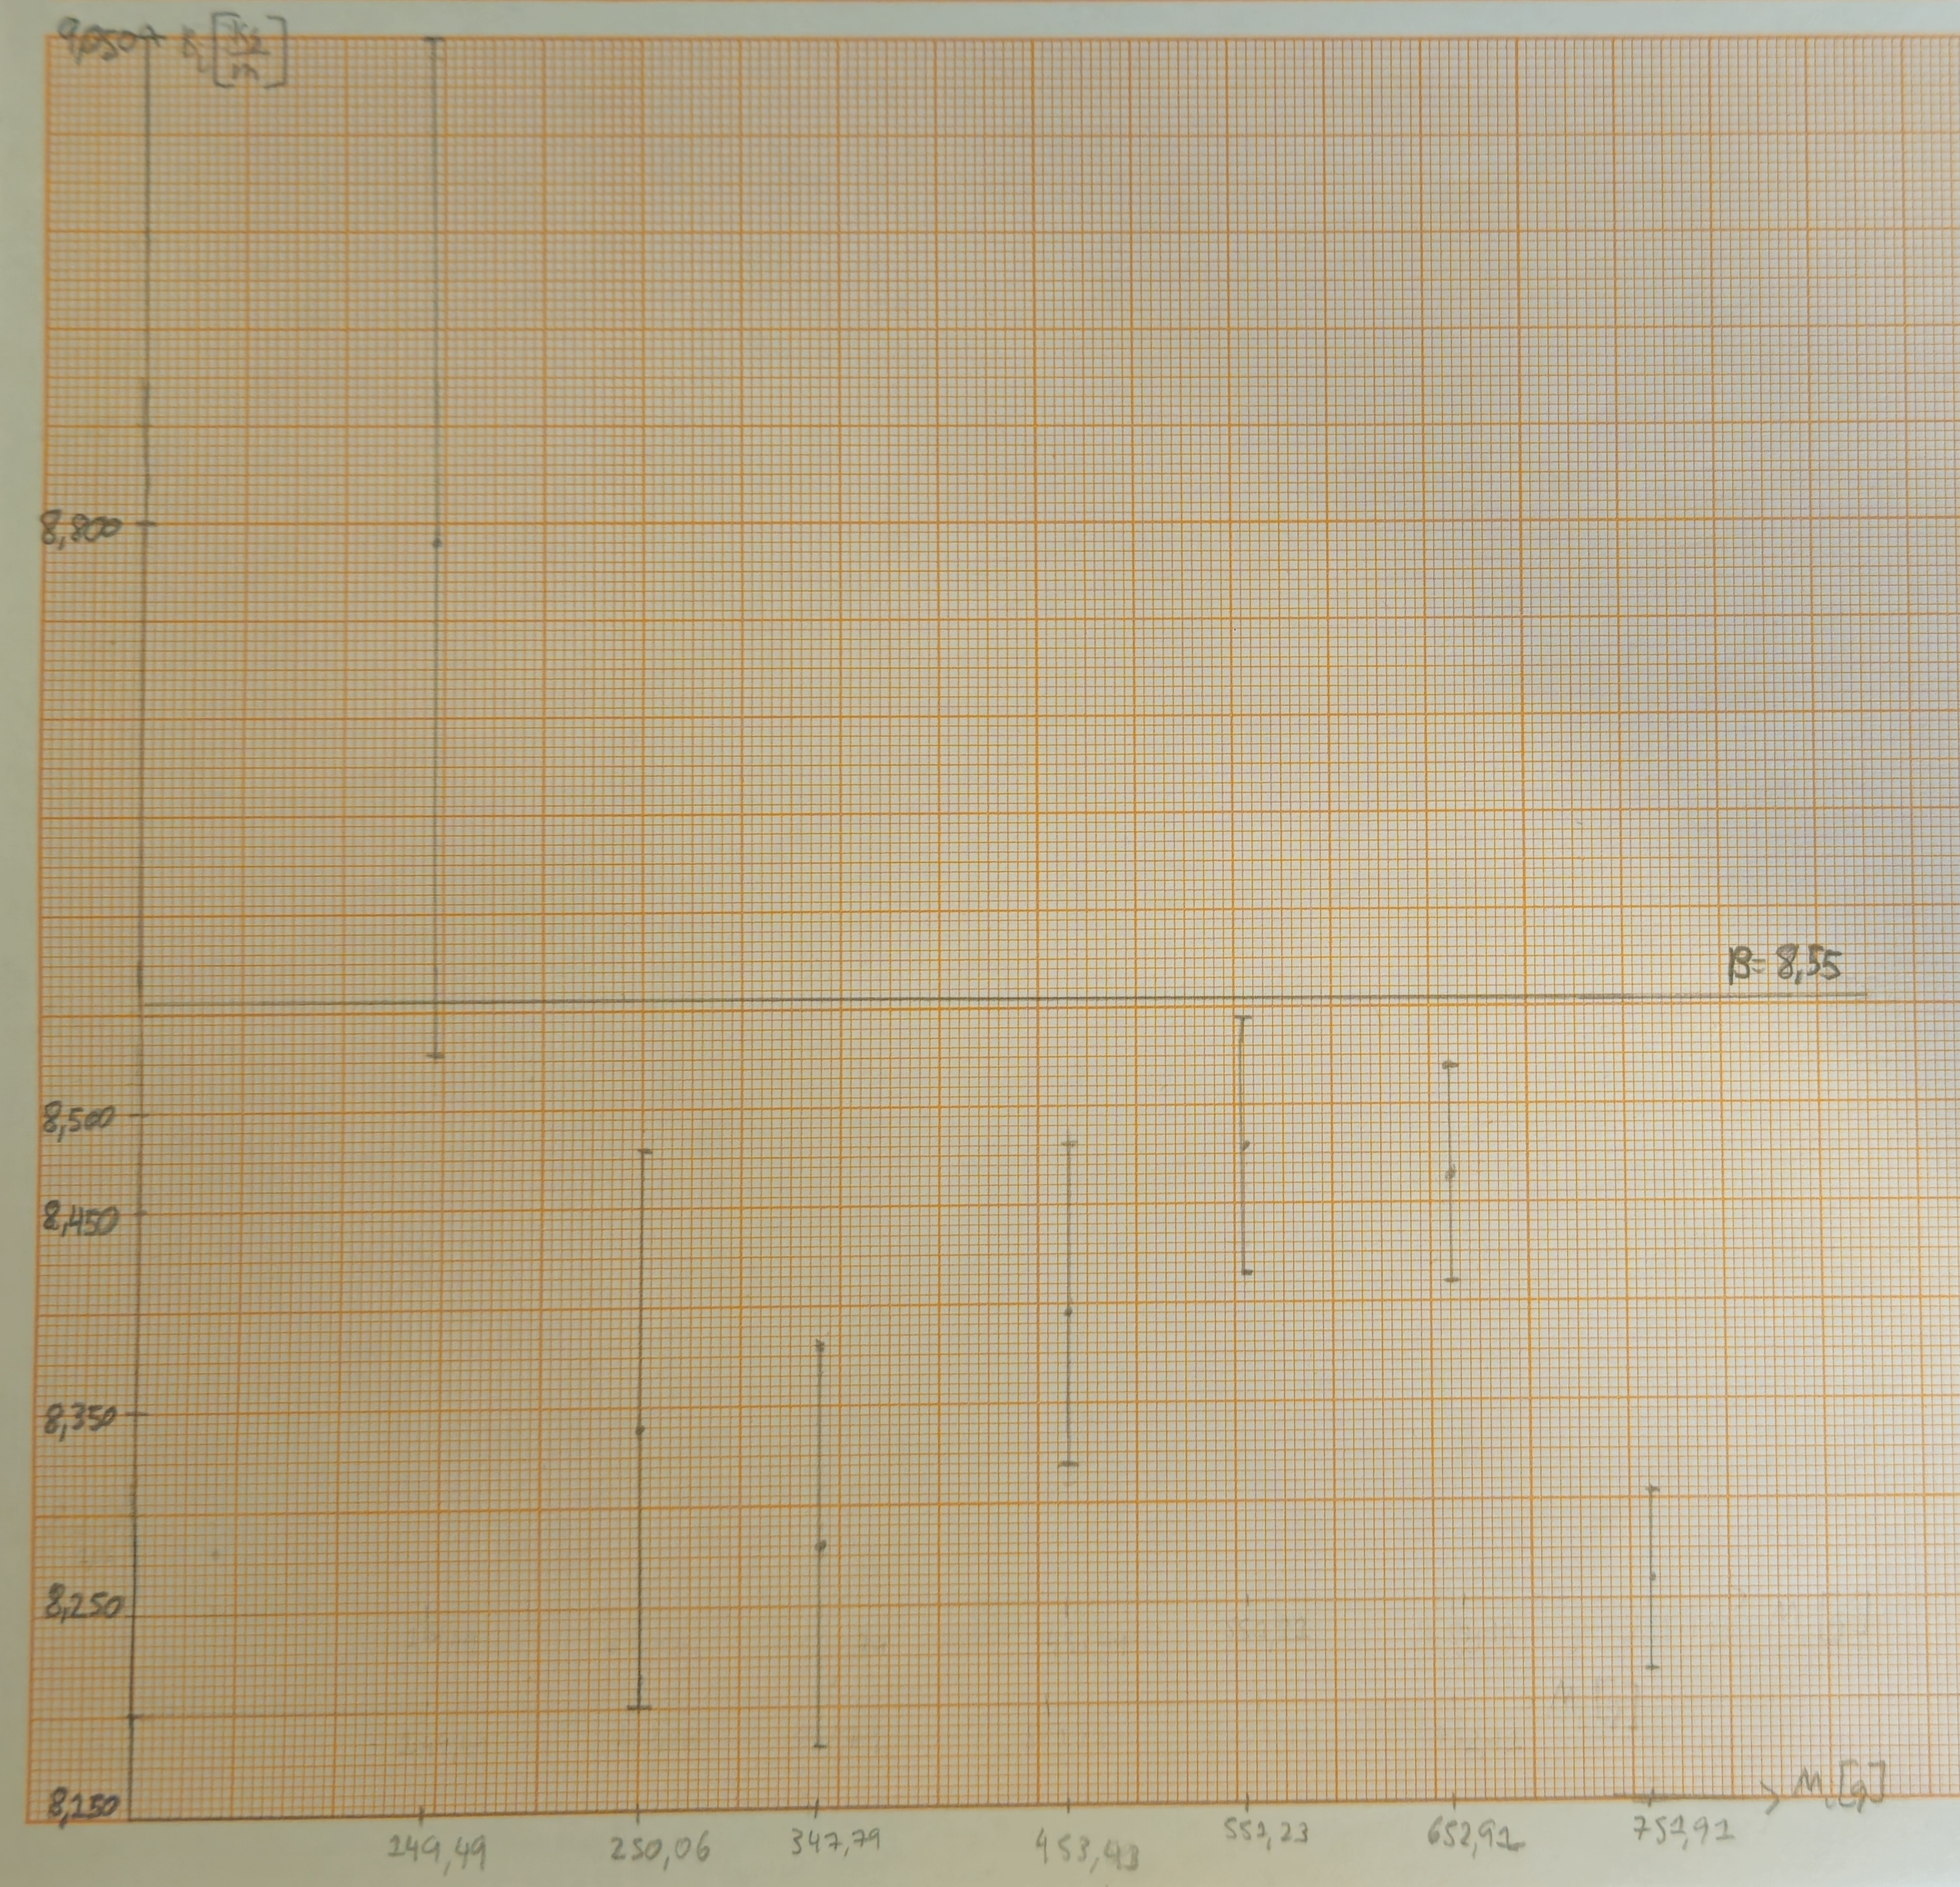
\includegraphics[width=0.8\textwidth]{fotoyoung/young_bi.jpg}
    \caption{Grafico di $B_i$ vs $M_i$}
\end{figure}

\end{document}
